%! TeX program = xelatex

\documentclass[xetex,aspectratio=169,xcolor,professionalfonts,hyperref]{beamer}
\usepackage[
    style=authoryear,
    backend=biber,
    natbib,
    uniquename=false,
    maxcitenames=2,
    maxbibnames=20,
    sorting=nty]{biblatex}
\addbibresource{refs.bib}
\renewcommand*{\bibfont}{\scriptsize}
\usepackage{anyfontsize}
\usepackage{tabularx}
\usepackage{changepage}
\usetheme{dark18}
\usepackage{stmaryrd}
\usepackage{nicefrac}
\usepackage{graphicx}
\usepackage{stackrel}
\usepackage{booktabs}
\usepackage{xspace}
\usepackage{tikz-dependency}
\usepackage{tkz-graph}
\usepackage{pgfplots}
\usepgfplotslibrary{groupplots}
% emojis!
\makeatletter
\newcommand*\fsize{\dimexpr\f@size pt\relax}
\makeatother
\newcommand*\emoji[2][1]{\includegraphics[width=#1\fsize]{emoji/#2}}
%
%% Generic TiKZ utils!
\usetikzlibrary{calc,backgrounds,arrows,arrows.meta}
\usetikzlibrary{decorations.pathreplacing}
\usetikzlibrary{tikzmark,positioning,patterns}
\usetikzlibrary{bending}
\usetikzlibrary{overlay-beamer-styles}
\pgfdeclarelayer{background}
\pgfdeclarelayer{foreground}
\pgfsetlayers{background,main,foreground}
%
\tikzset{
    visible on/.style={alt={#1{}{invisible}}},
    invisible/.style={opacity=0},
    alt/.code args={<#1>#2#3}{%
      \alt<#1>{\pgfkeysalso{#2}}{\pgfkeysalso{#3}} % \pgfkeysalso doesn't change the path
    },
  }

%% particular stuff?
\newcommand*{\ticksize}{2pt}
\tikzset{axisline/.style={thick,myfg!50!mybg,text=myfg,font=\small}}
\tikzset{axislabel/.style={font=\small}}
\tikzset{point/.style={thick,tMidnight}}


% semantic color definitions
\colorlet{colorArgmax}{tTarmac}
\colorlet{colorSoftmax}{tVividBlue}
\colorlet{colorSparsemax}{tYellow!50}
\colorlet{colorFusedmax}{tPeony!80!mybg}
\colorlet{colorEntmax}{tPeony}


\tikzset{
    tinyarrowl/.style={-{Straight Barb[bend]},thick,bend left=75,tPeony},
    tinyarrowr/.style={-{Straight Barb[bend]},thick,bend right=75,tPeony}}
\newcommand{\miniparse}[1]{%
{\footnotesize%
\begin{tikzpicture}[
    node distance=14pt,
    every node/.style={inner sep=0,outer sep=1pt},
    ]
\node[tPeony] (a) at (0, 0) {\textbullet};
\node[tPeony,right of=a] (b) {\textbullet};
\node[tPeony,right of=b] (c) {\textbullet};
\foreach \i/\j/\r/\o in {#1}{
\path (\i.north) edge[tinyarrow\r,opacity=\o] (\j.north);
}\end{tikzpicture}}}

% Tikz pic: draw a cog
\tikzset{cog/.pic={code={
    \draw[myfg,thick,fill=tTarmac!90]
  (0:2)
  \foreach \i [evaluate=\i as \n using {(\i-1)*360/18}] in {1,...,18}{%
    arc (\n:\n+10:2) {[rounded corners=1.5pt] -- (\n+10+2:2.4)
    arc (\n+10+2:\n+360/18-2:2.4)} --  (\n+360/18:2)
  };
  \draw[myfg,thick,fill=mybg] (0,0) circle[radius=.5];
}}}
%
%
% Tikz: draw an envelope
\newsavebox\envelope
\savebox{\envelope}{

\newlength\mylen
\setlength\mylen{2cm}
\begin{tikzpicture}[scale=.65]

\coordinate (A) at (0,0);
\coordinate (B) at (1.41\mylen,-\mylen);
\clip
  ([xshift=-0.5\pgflinewidth,yshift=0.5\pgflinewidth]A) --
  ([xshift=0.5\pgflinewidth,yshift=0.5\pgflinewidth]A-|B) --
  ([xshift=0.5\pgflinewidth,yshift=-0.5\pgflinewidth]B) --
  ([xshift=-0.5\pgflinewidth,yshift=-0.5\pgflinewidth]B-|A) --
  ([xshift=-0.5\pgflinewidth,yshift=0.5\pgflinewidth]A);
\draw[mybg,fill=tTarmac,line cap=rect]
  (A) -- (A-|B) -- (B) -- (B-|A) -- (A);
\draw[mybg]
  (B-|A) -- (0.705\mylen,-.3\mylen) -- (B);
\draw[mybg,fill=tTarmac!90,rounded corners=15pt]
  (A) -- (0.705\mylen,-0.6\mylen) -- (A-|B);
\node[anchor=north]
  at ($ (A)!0.5!(B|-A) $ ) {\parbox{\mylen}{}};
\draw[mybg] (A) -- (B|-A);
\end{tikzpicture}
}
%
% output
\newsavebox\sentoutput
\savebox{\sentoutput}{%
    \begin{tikzpicture}[scale=.75,text=myfg]
 \draw[rounded corners,tTarmac!60,very thick] (-.5, -.5) rectangle (.5, 2.5) {};

 \node[label={[label distance=.25cm]0:positive}] (pos) at (0, 2) {};
 \node[label={[label distance=.25cm]0:neutral}] (neu) at (0, 1) {};
 \node[label={[label distance=.25cm]0:negative}] (neg) at (0, 0) {};

 \draw[fill=tNavy!80!myfg] (pos) circle[radius=9pt];
 \draw[fill=tNavy!20!myfg] (neu) circle[radius=9pt];
 \draw[fill=tNavy!20!myfg] (neg) circle[radius=9pt];
 \end{tikzpicture}
 }
%
% cartoon structure
\newcommand{\cartoon}[2][1]{%
\begin{tikzpicture}%
\node[draw=none, minimum size=#1*1cm, regular polygon, regular polygon sides=5] (p) {};
%
\foreach \i/\j in {#2}%
{
    \draw[tPeony, ultra thick] (p.corner \i) -- (p.corner \j);
}
%
\foreach \i in {1, ..., 5}%
{
    \draw[myfg,fill=mybg,very thick] (p.corner \i) circle[radius=#1*5pt];
}
\end{tikzpicture}}
\newcommand{\cartoonDense}[1][1]{%
\begin{tikzpicture}%
\node[draw=none, minimum size=#1*1cm, regular polygon, regular polygon sides=5] (p) {};
%
\draw[tPeony, ultra thick, opacity=.8] (p.corner 1) -- (p.corner 2);
\draw[tPeony, ultra thick, opacity=.5] (p.corner 1) -- (p.corner 3);
\draw[tPeony, ultra thick, opacity=.7] (p.corner 1) -- (p.corner 4);
\draw[tPeony, ultra thick, opacity=.4] (p.corner 1) -- (p.corner 5);
\draw[tPeony, ultra thick, opacity=.6] (p.corner 2) -- (p.corner 3);
\draw[tPeony, ultra thick, opacity=.3] (p.corner 2) -- (p.corner 4);
\draw[tPeony, ultra thick, opacity=.9] (p.corner 2) -- (p.corner 5);
\draw[tPeony, ultra thick, opacity=.2] (p.corner 3) -- (p.corner 4);
\draw[tPeony, ultra thick, opacity=.6] (p.corner 3) -- (p.corner 5);
\draw[tPeony, ultra thick, opacity=.4] (p.corner 4) -- (p.corner 5);
%
\foreach \i in {1, ..., 5}%
{
    \draw[myfg,fill=mybg,very thick] (p.corner \i) circle[radius=#1*5pt];
}
\end{tikzpicture}}
\newcommand{\cartoonSparse}[1][1]{%
\begin{tikzpicture}%
\node[draw=none, minimum size=#1*1cm, regular polygon, regular polygon sides=5] (p) {};
%
\draw[tPeony, ultra thick, opacity=1] (p.corner 1) -- (p.corner 4);
\draw[tPeony, ultra thick, opacity=.5] (p.corner 2) -- (p.corner 5);
\draw[tPeony, ultra thick, opacity=.5] (p.corner 1) -- (p.corner 5);
%
\foreach \i in {1, ..., 5}%
{
    \draw[myfg,fill=mybg,very thick] (p.corner \i) circle[radius=#1*5pt];
}
\end{tikzpicture}}
%
\newcommand{\setupsimplexbary}[1][3.3]{%
\coordinate (L1) at (0:0);
\coordinate (L2) at (0:#1);
\coordinate (L3) at (60:#1);

\node[label=east:{\small$\triangle$}] at (L2) {};

\fill[tYellow,opacity=.15]  (L1) -- (L2) -- (L3) -- cycle;
\draw[very thick,tYellow] (L1) -- (L2) -- (L3) -- cycle;

\draw[tYellow,fill] (L1) circle[radius=3pt];
\draw[tYellow,fill] (L2) circle[radius=3pt];
\draw[tYellow,fill] (L3) circle[radius=3pt];
}

\newcommand{\drawcs}{%
\node[anchor=south] at (0, \vecheight*4) {$c_1$};
\node[anchor=south] at (0, \vecheight*3) {$c_2$};
\node[anchor=south] at (0, \vecheight*1.5) {$\cdots$};
\node[anchor=south] at (0, \vecheight*0) {$c_N$};}

\newcommand{\drawscores}{%
\node[anchor=south] at (-1-.5*\vecwidth, \vecheight*5+.1) {$\s$};
\draw[elem,fill=vecfg!60!vecbg] (-1-\vecwidth, \vecheight*4) rectangle (-1, \vecheight*5);
\draw[elem,fill=vecfg!85!vecbg] (-1-\vecwidth, \vecheight*3) rectangle (-1, \vecheight*4);
\draw[elem,fill=vecfg!60!vecbg] (-1-\vecwidth, \vecheight*2) rectangle (-1, \vecheight*3);
\draw[elem,fill=vecfg!75!vecbg] (-1-\vecwidth, \vecheight*1) rectangle (-1, \vecheight*2);
\draw[elem,fill=vecfg!50!vecbg] (-1-\vecwidth, \vecheight*0) rectangle (-1, \vecheight*1);
}

\newcommand{\drawargmax}{%
\node[anchor=south] at (1+.5*\vecwidth, \vecheight*5+.1) {$\p$};
\draw[elem,fill=vecfg! 0!vecbg]  (1, \vecheight*4) rectangle (1+\vecwidth, \vecheight*5);
\draw[elem,fill=vecfg!70!vecbg]  (1, \vecheight*3) rectangle (1+\vecwidth, \vecheight*4);
\draw[elem,fill=vecfg! 0!vecbg]  (1, \vecheight*2) rectangle (1+\vecwidth, \vecheight*3);
\draw[elem,fill=vecfg! 0!vecbg]  (1, \vecheight*1) rectangle (1+\vecwidth, \vecheight*2);
\draw[elem,fill=vecfg! 0!vecbg]  (1, \vecheight*0) rectangle (1+\vecwidth, \vecheight*1);
}
\newcommand{\drawsoftmax}{%
\node[anchor=south] at (1+.5*\vecwidth, \vecheight*5+.1) {$\p$};
\draw[elem,fill=vecfg!30!vecbg]  (1, \vecheight*4) rectangle (1+\vecwidth, \vecheight*5);
\draw[elem,fill=vecfg!50!vecbg]  (1, \vecheight*3) rectangle (1+\vecwidth, \vecheight*4);
\draw[elem,fill=vecfg!35!vecbg]  (1, \vecheight*2) rectangle (1+\vecwidth, \vecheight*3);
\draw[elem,fill=vecfg!25!vecbg]  (1, \vecheight*1) rectangle (1+\vecwidth, \vecheight*2);
\draw[elem,fill=vecfg!15!vecbg]  (1, \vecheight*0) rectangle (1+\vecwidth, \vecheight*1);
}


% math and notation
\newcommand*\bs[1]{\boldsymbol{#1}}
\newcommand\defeq{{\,\raisebox{1pt}{$:$}=}\,}
\newcommand\p{\bs{p}}
\newcommand\xx{z}
\newcommand\x{\bs{\xx}}
\newcommand\s{\x}
\renewcommand\ss{\xx}
\newcommand\mg{\bs{\mu}}
\newcommand\pr{\bs{\eta}}
\newcommand\Mp{\mathcal{M}}
\newcommand\parp{\bs{\pi}}
\newcommand\clfp{\bs{\phi}}
\DeclareMathOperator*{\argmax}{arg\,max}
\DeclareMathOperator*{\argmin}{arg\,min}
\DeclareMathOperator{\HH}{H}
\DeclareMathOperator{\mapo}{\bs{\pi}_{\Omega}}
\DeclareMathOperator{\diag}{diag}
\DeclareMathOperator{\ident}{Id}
\DeclareMathOperator{\dom}{dom}
\DeclareMathOperator{\conv}{conv}
\newcommand\reals{\mathbb{R}}

\newcommand{\pfrac}[2]{\frac{\partial #1}{\partial #2}}
\newcommand{\langp}[2]{\textsc{#1}$\shortrightarrow$\textsc{#2}}
\newcommand{\langpb}[2]{\textsc{#1}$\leftrightarrow$\textsc{#2}}
\newcommand*\entmaxtext{entmax\xspace}
\DeclareMathOperator*{\entmax}{\mathsf{\entmaxtext}}
\newcommand*\aentmax[1][\alpha]{\mathop{\mathsf{#1}\textnormal{-}\mathsf{\entmaxtext}}}
\DeclareMathOperator*{\softmaxlight}{\mathsf{softmax}}

% smaller and gray citation
\let\realcitep\citep
\renewcommand*{\citep}[1]{{\color{mygr}\scriptsize\realcitep{#1}}}
\newcommand*{\citeparg}[2]{{\color{mygr}\scriptsize\parencite[][#2]{#1}}}

\usepackage{etoolbox}
\usepackage{fp}
\makeatletter
\newcounter{ROWcellindex@}
\newtoggle{@doneROWreads}
\newcommand\setstackEOL[1]{%
  \ifstrempty{#1}{\def\SEP@char{ }}{\def\SEP@char{#1}}%
  \expandafter\define@processROW\expandafter{\SEP@char}%
}
\newcommand\define@processROW[1]{%
    \def\@processROW##1#1##2||{%
      \def\@preSEP{##1}%
      \def\@postSEP{##2}%
    }%
}
\newcommand\getargs[1]{%
  \togglefalse{@doneROWreads}%
  \edef\@postSEP{\unexpanded{#1}\expandonce{\SEP@char}}%
  \setcounter{ROWcellindex@}{0}%
  \whileboolexpr{test {\nottoggle{@doneROWreads}}}{%
    \stepcounter{ROWcellindex@}%
    \expandafter\@processROW\@postSEP||%
    \expandafter\ifstrempty\expandafter{\@postSEP}{%
      \toggletrue{@doneROWreads}%
    }{}%
    \csedef{arg\roman{ROWcellindex@}}{\expandonce{\@preSEP}}%
  }%
% \narg GIVES HOW MANY ROWS WERE PROCESSED
  \xdef\narg{\arabic{ROWcellindex@}}%
}
\makeatother
\setstackEOL{,}

\usepackage{ifthen}

\newcounter{index}
\newcommand\makearglist[2]{%
  \def\arglist{}%
  \getargs{#1}%
  \setcounter{index}{\narg}%
  \addtocounter{index}{-1}%
  \FPdiv\dTHETA{270}{\theindex}%
  \setcounter{index}{0}%
  \whiledo{\theindex<\narg}{%
    \FPmul\THETA{\theindex}{\dTHETA}%
    \stepcounter{index}%
    \def\thislabel{$\csname arg\roman{index}\endcsname$}%
    \edef\arglist{\arglist -45+\THETA / \thislabel}%
    \ifthenelse{\equal{\theindex}{\narg}}{}{\edef\arglist{\arglist,}}%
  }%
  \FPsub\pointdif{#2}{\argi}%
  \FPsub\DELTA{\argii}{\argi}%
  \FPdiv\NUMticks{\pointdif}{\DELTA}%
  \FPmul\DEGticks{\NUMticks}{\dTHETA}%
  \FPadd\POINTangle{-45}{\DEGticks}%
}

\newcommand\drawdial[2]{%
\makearglist{#1}{#2}%
\begin{tikzpicture}
  \draw[ultra thick] (0,0) circle [radius=0.5];
  \foreach \angle/\label in \arglist
  {
    \draw +(\angle:0.25) -- +(\angle:0.5);
    \draw (\angle:0.85) node {\label};
  }
  \draw[ultra thick] (0,0) -- +(\POINTangle:0.5);
%
\end{tikzpicture}%
}

\tikzset{
  every overlay node/.style={
    draw=black,fill=white,rounded corners,anchor=north west,
  },
}
% Usage:
% \tikzoverlay at (-1cm,-5cm) {content};
% or
% \tikzoverlay[text width=5cm] at (-1cm,-5cm) {content};
\def\tikzoverlay{%
   \tikz[baseline,overlay]\node[every overlay node];
}%
%%\usepackage{sectsty}
%%\subsubsectionfont{\normalfont\underline}
%\usepackage[explicit]{titlesec}
%\usepackage[normalem]{ulem}
%\titleformat{\subsubsection}{\normalfont}{\thesubsubsection}{1em}{\uline{#1}}
%%\titleformat{\subsection}{\normalfont}{\thesubsection}{1em}{\bf{#1}}
%
%\usepackage[font=footnotesize]{caption}
%\usepackage[font=small]{caption}
%\usepackage{sidecap}
%\usepackage{wrapfig}
%
%\usepackage{multirow}

%\newtheorem{theorem}{Theorem}
%\newtheorem{definition}[theorem]{\bf{Definition}}
\newtheorem{proposition}[theorem]{\bf{Proposition}}
%\newtheorem{lemma}[theorem]{\bf{Lemma}}
%\newtheorem{corollary}[theorem]{\bf{Corollary}}
%\newtheorem{example}[theorem]{\bf{Example}}
\newtheorem{remark}[theorem]{\bf{Remark}}
\newtheorem{property}[theorem]{\bf{Property}}
\newtheorem{procedure}[theorem]{\bf{Procedure}}



% % "box" symbols at end of proofs
\def\QEDclosed{\mbox{\rule[0pt]{1.3ex}{1.3ex}}} % for a filled box
% V1.6 some journals use an open box instead that will just fit around a closed one
\def\QEDopen{{\setlength{\fboxsep}{0pt}\setlength{\fboxrule}{0.2pt}\fbox{\rule[0pt]{0pt}{1.3ex}\rule[0pt]{1.3ex}{0pt}}}}
\def\QED{\QEDclosed} % default to closed
\def\proof{\noindent\hspace{0em}{\itshape Proof: }}
\def\endproof{\hspace*{\fill}~\QED\par\endtrivlist\unskip}
\def\lemmaproof{\noindent\hspace{0em}{\itshape Proof (of the Lemma): }}
\def\endlemmaproof{\hspace*{\fill}~\QED\par\endtrivlist\unskip}


%\newcommand{\Prob}[1]{\prob\{#1\}}
\newcommand{\Prob}{\mathbb{P}}

\newcommand{\vect}[1]{\mathbf{#1}}
\newcommand{\set}[1]{\mathbb{#1}}
\newcommand{\sett}[1]{\mathcal{#1}}
%\newcommand{\sett}[1]{{#1}}
\newcommand{\vectsymb}[1]{\boldsymbol{#1}}
\newcommand{\vectsymbscript}[1]{\boldsymbol{#1}}
%\newcommand{\vectsymb}[1]{\mbox{\boldmath$#1$}}
%\newcommand{\vectsymbscript}[1]{\mbox{{\scriptsize\boldmath$#1$}}}
\newcommand{\tup}[1]{\mathscr{#1}}
%\newcommand{\tup}[1]{\mathcal{#1}}
\newcommand{\sembrack}[1]{[\![#1]\!]}

\newcommand{\y}{{\vectsymb{y}}}
\newcommand{\z}{{\vectsymb{z}}}
\newcommand{\hh}{{\vectsymb{h}}}
\newcommand{\sss}{{\vectsymb{s}}}
\newcommand{\aaa}{{\vectsymb{a}}}
\newcommand{\bb}{{\vectsymb{b}}}
\newcommand{\X}{{\matr{X}}}
\newcommand{\Y}{{\matr{Y}}}
\newcommand{\Z}{{\matr{Z}}}
\newcommand{\SSS}{{\matr{S}}}

\newcommand{\W}{{\vectsymb{w}}}
\newcommand{\F}{{\vectsymb{f}}}
\newcommand{\w}{{w}}
\newcommand{\f}{{f}}
\newcommand{\B}{{\vectsymb{b}}}
\newcommand{\Score}{\vectsymb{\theta}}
\newcommand{\score}{{\theta}}
\newcommand{\DP}[2]{{#1}^{\top}{#2}}
%\newcommand{\DP}[2]{{#1}\cdot{#2}}
\newcommand{\Reg}{\Omega}
\newcommand{\Loss}{L}
\newcommand{\Scorepart}{\phi}
%\newcommand{\MARG}{\sett{M}}
\newcommand{\MARG}{\mathrm{MARG}}
%\newcommand{\LOCAL}{\sett{L}}
\newcommand{\LOCAL}{\mathrm{LOCAL}}


\newcommand{\bigforallandall}[2]{\underset{\substack{{#1}\\{#2}}}{\text{\LARGE{$\forall$}}}}
\newcommand{\bigforall}[1]{\underset{#1}{\text{\LARGE{$\forall$}}}}
\newcommand{\bigexistsandexists}[2]{\underset{\substack{{#1}\\{#2}}}{\text{\LARGE{$\exists$}}}}
\newcommand{\bigexists}[1]{\underset{#1}{\text{\LARGE{$\exists$}}}}
\newcommand{\bigvarepsilon}{\mbox{\large$\varepsilon$}}

\newcommand{\elide}[1]{{\emph{\textcolor{blue}{#1}}}}

\DeclareMathOperator{\csoftmax}{\mathbf{csoftmax}}
\DeclareMathOperator{\csparsemax}{\mathbf{csparsemax}}
\DeclareMathOperator{\affine}{\mathsf{affine}}
\DeclareMathOperator{\concat}{\mathsf{concat}}

\DeclareMathOperator{\card}{\mathtt{card}}
\DeclareMathOperator{\rank}{\mathtt{rank}}
\DeclareMathOperator{\BlkDiag}{\mathtt{BlkDiag}}
\DeclareMathOperator{\Diag}{\mathtt{Diag}}
\DeclareMathOperator{\epi}{\mathtt{epi}}
\DeclareMathOperator{\hypo}{\mathtt{hypo}}
\DeclareMathOperator{\image}{\mathtt{Im}}
\DeclareMathOperator{\kernel}{\mathtt{Ker}}
\DeclareMathOperator{\relint}{\mathtt{ri}}
\DeclareMathOperator{\interior}{\mathtt{int}}
\DeclareMathOperator{\proj}{\mathtt{Proj}}
\DeclareMathOperator{\co}{\mathtt{co}}
\DeclareMathOperator{\volume}{\mathtt{vol}}

\DeclareMathOperator*{\argmaxbf}{\mathbf{argmax}}
\DeclareMathOperator*{\Argmax}{Argmax}
\DeclareMathOperator*{\Argmin}{Argmin}
\DeclareMathOperator*{\argsup}{argsup}
\DeclareMathOperator*{\arginf}{arginf}
\DeclareMathOperator*{\Argsup}{Argsup}
\DeclareMathOperator*{\Arginf}{Arginf}
\DeclareMathOperator*{\sgn}{sgn}

\renewcommand{\exp}{\mathsf{exp}}
\renewcommand{\tanh}{\mathsf{tanh}}
\renewcommand{\log}{\mathsf{log}}
%\renewcommand{\min}{\mathsf{min}}
%\DeclareMathOperator*{\max}{\mathsf{max}}


\newenvironment{itemizesquish}{\begin{list}{\labelitemi}{\setlength{\itemsep}{0em}\setlength{\labelwidth}{0.5em}\setlength{\leftmargin}{\labelwidth}\addtolength{\leftmargin}{\labelsep}}}{\end{list}}


\newenvironment{enumeratesquish}{\begin{list}{\addtocounter{enumi}{1}\labelenumi}{\setlength{\itemsep}{0em}\setlength{\labelwidth}{0.5em}\setlength{\leftmargin}{\labelwidth}\addtolength{\leftmargin}{\labelsep}}}{\end{list}\setcounter{enumi}{0}}


\newcommand{\dataset}{{\cal D}}
\newcommand{\fracpartial}[2]{\frac{\partial #1}{\partial  #2}}

\newcommand{\correct}[1]{{\color{blue}{\it #1}}}
\newcommand{\wrong}[1]{{\color{red}{\bf #1}}}
\newcommand{\source}[1]{{\textcolor{olive}{#1}}}
\captionsetup[figure]{labelformat=empty}
\pgfplotsset{compat=1.16}
\newcommand\simplex{\triangle}
\newcommand\HHs{\HH^{\textsc{s}}}
\newcommand\HHg{\HH^{\textsc{g}}}
\newcommand\HHta{\HH^{\textsc{t}}_{\alpha}}
\newcommand\xv{\bs{x}}
\newcommand{\matr}[1]{\mathbf{#1}}
\DeclareMathOperator{\softmax}{\mathbf{softmax}}
\DeclareMathOperator{\sparsemax}{\mathbf{sparsemax}}
\definecolor{tBleu}{RGB}{118,169,196}
\definecolor{tDY}{RGB}{217,192,102}
\title{Efficient Marginalization of Discrete and Structured Latent Variables via Sparsity}
\author{Gonçalo Correia, Vlad Niculae, Andr\'{e} F.T. Martins}

\addtobeamertemplate{navigation symbols}{}{%
    \usebeamerfont{footline}%
    \usebeamercolor[fg]{footline}%
    \hspace{1em}%
    \insertframenumber/\inserttotalframenumber
}

% \AtBeginSection[]
% {
% \begin{frame}
%     \frametitle{Table of Contents}

%     \begin{adjustwidth}{5cm}{0.1em}
%         \tableofcontents[currentsection]
%     \end{adjustwidth}
% \end{frame}
% }

\begin{document}

\begin{frame}
%\titlepage
\begin{tikzpicture}[remember picture, overlay]

\node[font={\color{myfg}\usebeamerfont{title}},align=center]
    at ($(current page.center) + (0, 2.5)$) {\color{myDarkYellow} Efficient Marginalization};
\node[font={\color{myfg}\usebeamerfont{title}},align=center]
    at ($(current page.center) + (0, 1.8)$) {\color{myDarkYellow} of Discrete and Structured Latent Variables};
\node[font={\color{myfg}\usebeamerfont{title}},align=center]
    at ($(current page.center) + (0, 1.0)$) {\color{myDarkYellow} via Sparsity};
\node[anchor=north,font={\color{myfg}\usebeamerfont{author}}]
    at ($(current page.center) + (0, 0.5)$)
{
\renewcommand{\arraystretch}{1.5}
\begin{tabular}{r l}
\textbf{Gonçalo Correia} &\small \textcolor{mygr}{Instituto de Telecomunicações, Lisbon} \\
Vlad Niculae             &\small \textcolor{mygr}{IvI, University of Amsterdam} \\
Wilker Aziz             &\small \textcolor{mygr}{ILLC, University of Amsterdam} \\
André Martins            &\small \textcolor{mygr}{Instituto de Telecomunicações \& LUMLIS \& Unbabel}  \\
\end{tabular}
};

\node[anchor=south,font={\color{mygr}\footnotesize}]
    at (current page.south)
{
\raisebox{-0.7mm}[\height][\depth]{\emoji{githubfg}} \href{https://github.com/deep-spin/sparse-marginalization-lvm}{\tt github.com/deep-spin/sparse-marginalization-lvm}
\quad
\raisebox{-0.4mm}[\height][\depth]{\emoji{home}}
\href{https://goncalomcorreia.github.io}{\tt goncalomcorreia.github.io}
};
\end{tikzpicture}
\end{frame}

\tikzset{%
    enc/.style={fill=tPurple!80!mybg},
    attn/.style={fill=tPeony},
    dec/.style={fill=tBlue!50!mybg},
    wvec/.style={
        inner sep=0,
        rectangle,
        rounded corners=2pt,
        minimum width=5pt,
        minimum height=18pt},
    word/.style={
        color=mygr,
        font=\itshape
    },
    netarrow/.style={->, color=mygr},
    attnedge/.style={tPeony, thick}
}

\section{Context}

\begin{frame}
    \frametitle{Latent Variable Models}

    \begin{itemize}
        \uncover<1->{\item[] Latent variable $z$ can be }\uncover<2->{{\color{tGreen} continuous}}\uncover<3->{, {\color{tPeony} discrete}}\uncover<4->{, or {\color{tVividBlue} structured}}
    \end{itemize}
    
    \only<1-2>{\uncover<2>{
    \begin{figure}[hb]
        \centering
        \begin{subfigure}[b]{0.24\columnwidth}
            \centering
            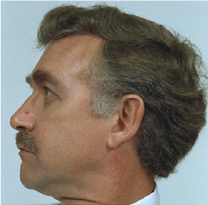
\includegraphics[width=\columnwidth]{figures/face1.png}
        \end{subfigure}
        \hfill
        \begin{subfigure}[b]{0.24\columnwidth}
            \centering
            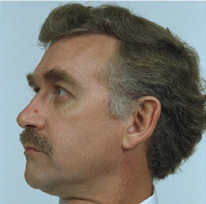
\includegraphics[width=\columnwidth]{figures/face2.png}
        \end{subfigure}
        \hfill
        \begin{subfigure}[b]{0.24\columnwidth}
            \centering
            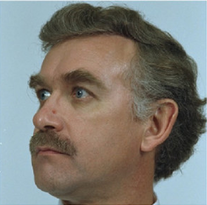
\includegraphics[width=\columnwidth]{figures/face3.png}
        \end{subfigure}
        \hfill
        \begin{subfigure}[b]{0.24\columnwidth}
            \centering
            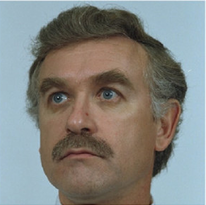
\includegraphics[width=\columnwidth]{figures/face4.png}
        \end{subfigure}
        \caption{Source: \cite{faces}}
        \label{fig:rotation}
    \end{figure}
    }}

    \only<3>{
    \begin{figure}[hb]
        \centering
            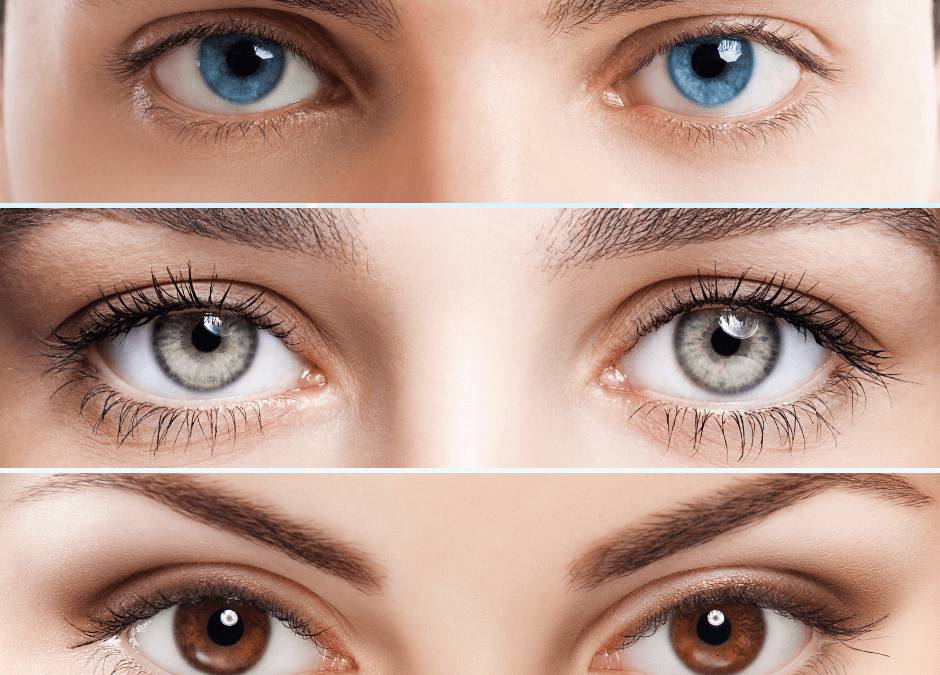
\includegraphics[width=0.5\columnwidth]{figures/eyes.png}
            \caption{Source: \href{https://valleyeyecareaz.com/how-is-your-eye-color-determined/}{valleyeyecareaz.com}}
        \label{fig:eyes}
    \end{figure}
    }

    \only<4>{
    \begin{figure}[hb]
        \centering
            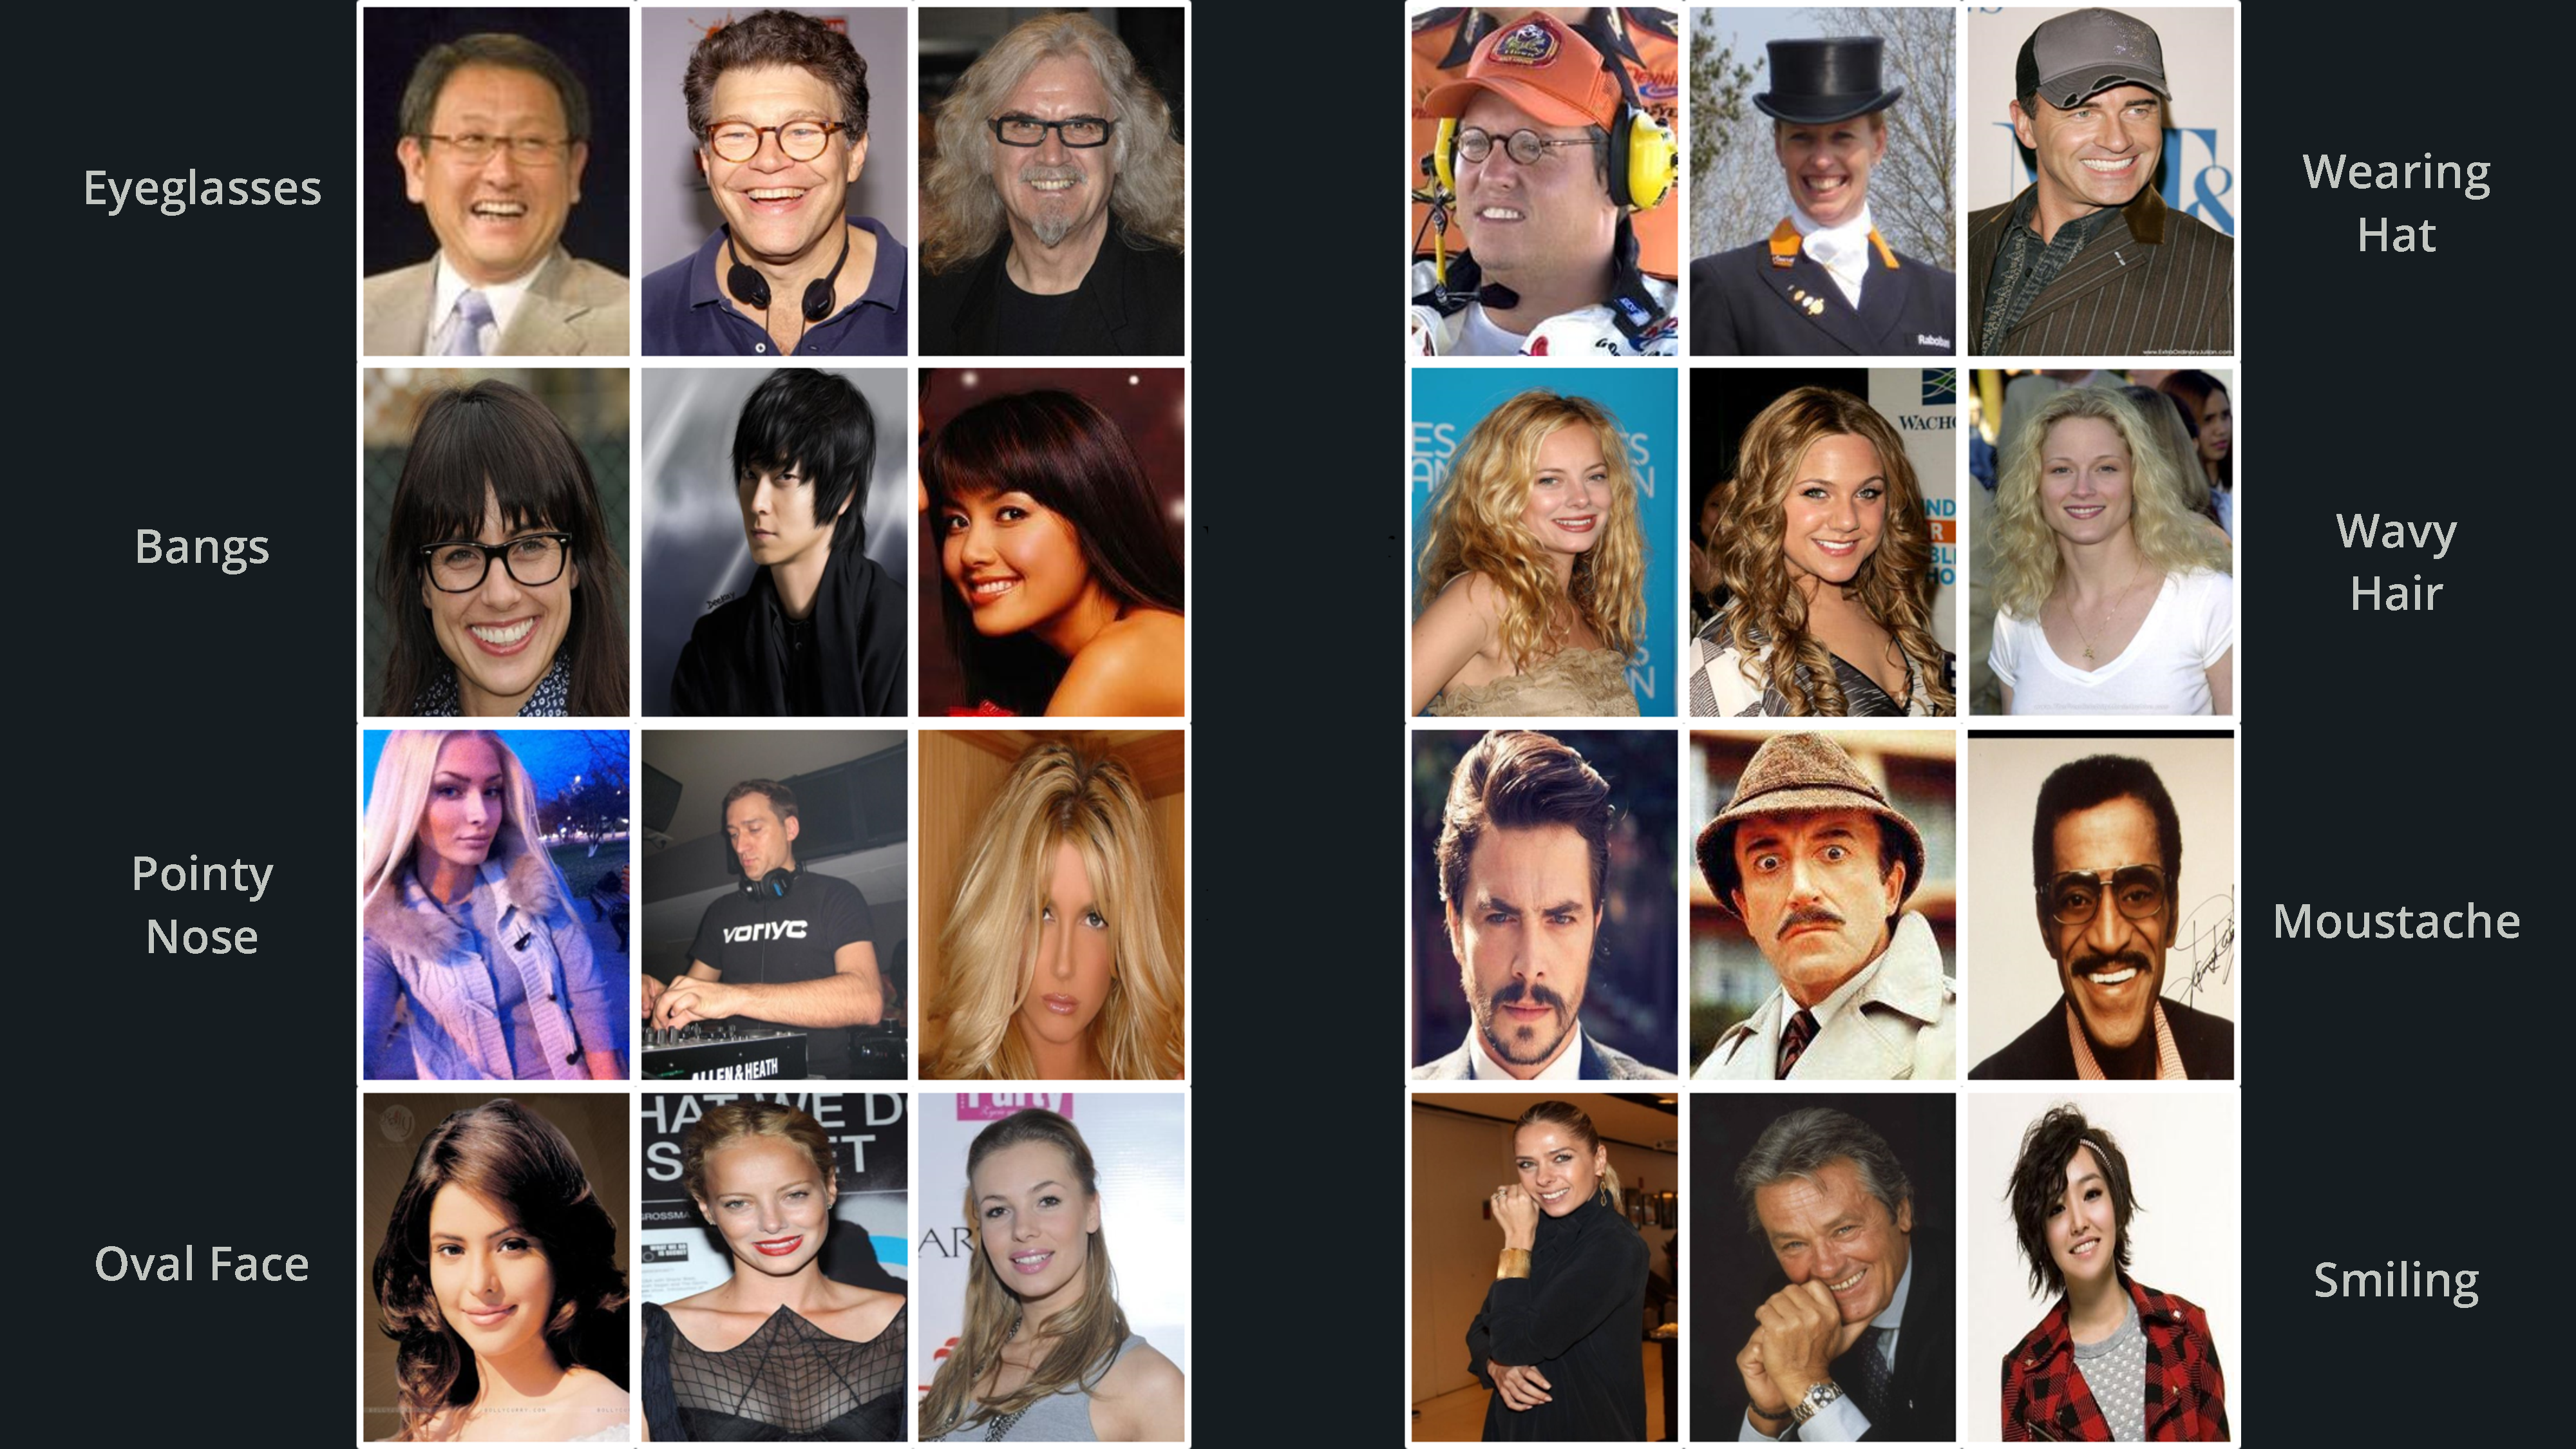
\includegraphics[width=0.6\columnwidth]{figures/celeba_bg.pdf}
            \caption{Source: \cite{liu2015faceattributes}}
        \label{fig:eyes}
    \end{figure}
    }

\end{frame}

\begin{frame}
    \frametitle{Training Discrete or Structured Latent Variable Models}
    \fontsize{12pt}{15}\selectfont

    \begin{columns}
    \hspace{2mm}\vspace{-1cm}\begin{column}{0.7\columnwidth}\vspace{-1cm}
    \begin{itemize}
        \uncover<1->{\item[] Latent variable $z$ can be }\uncover<2->{{\color{tPeony} discrete}}\uncover<3->{ or {\color{tVividBlue} structured}}
    \end{itemize}

    \begin{itemize}
        \uncover<4->{\item[] $\pi(z | x, \theta)$: distribution over possible $z$}
    \end{itemize}

    % besides this, there's also
    \begin{itemize}
        \uncover<7->{\item[] $\ell(x, z; \theta)$: downstream loss: ELBO, Log-Likelihood, (...)}
    \end{itemize}

    \end{column}

    \begin{column}{0.25\columnwidth}
            \vspace{-0.5cm}
            \begin{center}
                \begin{figure}[ht]
                \begin{tikzpicture}
                    % DISCRETE
                    \uncover<2->{\draw[draw=tPink,fill=tPink] (1.4,2) circle (0.2) node[anchor=south, yshift=2mm] {{\visible<5->{\color{tPeony} \small 0.2}}};}
                    \uncover<2->{\draw[draw=tSlateBlue,fill=tSlateBlue] (2,2) circle (0.2) node[anchor=south, yshift=2mm] {{\visible<5->{\color{tPeony} \small 0.6}}};}
                    \uncover<2->{\draw[draw=tGreen,fill=tGreen] (2.6,2) circle (0.2) node[anchor=south, yshift=2mm] {{\visible<5->{\color{tPeony} \small 0.1}}};}

                    % STRUCTURE
                    \uncover<3->{\draw[draw=tSlateBlue,fill=tSlateBlue] (1.4,1) circle (0.2) node[anchor=east, xshift=-2mm] {$[$};}
                    \uncover<3->{\draw[draw=tGreen,fill=tGreen] (2,1) circle (0.2);}
                    \uncover<3->{\draw[draw=tPink,fill=tPink] (2.6,1) circle (0.2)
                        node[anchor=west, xshift=2mm] {$]$}
                        node[anchor=west, xshift=5mm] {{\visible<6->{\color{tVividBlue} \small 0.4}}};}

                    \uncover<3->{\draw[draw=tPink,fill=tPink] (1.4,0.5) circle (0.2) node[anchor=east, xshift=-2mm] {$[$};}
                    \uncover<3->{\draw[draw=tSlateBlue,fill=tSlateBlue] (2,0.5) circle (0.2) node[anchor=north, yshift=-4mm] {\large \bf $\ldots$};}
                    \uncover<3->{\draw[draw=tGreen,fill=tGreen] (2.6,0.5) circle (0.2)
                        node[anchor=west, xshift=2mm] {$]$}
                        node[anchor=west, xshift=5mm] {{\visible<6->{\color{tVividBlue} \small 0.05}}};}

                    \uncover<3->{\draw[draw=tGreen,fill=tGreen] (1.4,-0.5) circle (0.2) node[anchor=east, xshift=-2mm] {$[$};}
                    \uncover<3->{\draw[draw=tSlateBlue,fill=tSlateBlue] (2,-0.5) circle (0.2);}
                    \uncover<3->{\draw[draw=tPink,fill=tPink] (2.6,-0.5) circle (0.2)
                        node[anchor=west, xshift=2mm] {$]$}
                        node[anchor=west, xshift=5mm] {{\visible<6->{\color{tVividBlue} \small 0.3}}};}
                \end{tikzpicture}
                \end{figure}
            \end{center}
    \end{column}
    \end{columns}

    \vspace{-0.5cm}

    \begin{itemize}
        \uncover<8->{\item[] To train, we need to compute the following expectation:}
    \end{itemize}

    \begin{equation*}\label{eq:fit}
        \uncover<9->{\mathcal{L}_{x}(\theta) =
        \sum_{z \in \mathcal Z}
        \pi(z | x, \theta)
        ~\ell(x, z; \theta)}
    \end{equation*}

    \begin{itemize}
        \uncover<10->
        {\item[] If $\mathcal Z$ is
        \only<10>{{\color{tPeony} large}, this sum can get very expensive due to $\ell(x, z; \theta)$!\quad\emoji{oface}}
        \only<11->{{\color{tVividBlue} combinatorial}, this can be intractable to compute!\quad\emoji{oface}\enspace\emoji{oface}\enspace\emoji{oface}}}
    \end{itemize}

\end{frame}

\begin{frame}
    \frametitle{Current Solutions}
    \fontsize{12pt}{15}\selectfont

    \begin{itemize}
        \item[] If $\mathcal Z$ is large, exact gradient computation is prohibitive
    \end{itemize}

    \bigskip

    \begin{itemize}
        \uncover<2->{\item[] One option: SFE (aka REINFORCE)---unbiased but high variance}
        \uncover<3->{\item[] Another option: Gumbel-Softmax---continuous relaxation, biased estimation}
    \end{itemize}

    \bigskip

    \begin{itemize}
        \uncover<4->{\item[] New option: {\color{tPeony} use sparsity}!\quad\emoji{palms}}
    \end{itemize}

    \begin{itemize}
        \uncover<5->{\item[] no need for sampling --> no variance}
        \uncover<6->{\item[] no relaxation into the continuous space}
    \end{itemize}
\end{frame}

\begin{frame}
    \frametitle{Taking a step back...}
    \fontsize{14pt}{15}\selectfont
    \begin{itemize}
        \item[] Does the expectation over possible $z$ need to be expensive?
    \end{itemize}

    \begin{align*}\label{eq:fit}
        \uncover<2->{\mathcal{L}_{x}(\theta) &=
        \sum_{z \in \mathcal Z}
        \pi(z | x, \theta)~\ell(x, z; \theta) \\&=
        \pi(z_1 | x, \theta)~\ell(x, z_1; \theta) + \pi(z_2 | x, \theta)~\ell(x, z_2; \theta) + \ldots \\&+ \pi(z_i | x, \theta)~\ell(x, z_i; \theta) + \ldots + \pi(z_N | x, \theta)~\ell(x, z_N; \theta)
        }
    \end{align*}

    % \begin{itemize}
    %     \uncover<3->{\item[] If components of $\pi(z | x, \theta)$ were exactly $0$, we could skip lots of computations!}
    % \end{itemize}

    \begin{itemize}
        \uncover<3->{\item[] Usually we normalize $\pi$ with softmax$\propto \exp(\pi) \Rightarrow \pi(z_i | x, \theta)>0$}
    \end{itemize}
\end{frame}

\begin{frame}
    \frametitle{Sparse normalizers}
    \fontsize{12pt}{15}\selectfont
    \cornercite[north east]{sparsemax, sparsemap}
    \begin{itemize}
        \item[] We use {\color{tPeony} sparsemax}, {\color{tVividBlue} top-$k$ sparsemax} and {\color{tVividBlue} SparseMAP} to allow efficient marginalization
    \end{itemize}

    \begin{itemize}
        \uncover<2->{\item[] These functions are able to assign {\bf probabilities of exactly zero}!}
    \end{itemize}

    \begin{align*}
        \uncover<3->{\mathcal{L}_{x}(\theta) &=
        \sum_{z \in \mathcal Z}
        \pi(z | x, \theta)~\ell(x, z; \theta) \\&=
        \pi(z_1 | x, \theta)~\ell(x, z_1; \theta) + \alt<3>{\pi(z_2 | x, \theta)~\ell(x, z_2; \theta)}{\cancel{\pi(z_2 | x, \theta)~\ell(x, z_2; \theta)}} + \ldots \\&+
        \pi(z_i | x, \theta)~\ell(x, z_i; \theta) + \ldots + \alt<3>{\pi(z_N | x, \theta)~\ell(x, z_N; \theta)}{\cancel{\pi(z_N | x, \theta)~\ell(x, z_N; \theta)}}
        }
    \end{align*}

    \begin{itemize}
        \uncover<4->{\item[] No need for computing $\ell(x, z; \theta)$ for all $z \in \mathcal Z$!}
    \end{itemize}
\end{frame}

\begin{frame}
    \frametitle{Results}
    \fontsize{14pt}{15}\selectfont
    \begin{itemize}
        \uncover<1->{\item[] We test our methods for models with discrete latent variables,}
        \begin{itemize}
            \uncover<2->{\item Semi-Supervised VAE}
            \uncover<3->{\item Emergent communication}
        \end{itemize}
        \uncover<4->{\item[] but also in models with an exponentially large set of $\mathcal Z$,}
        \begin{itemize}
            \uncover<5->{\item Bit-vector VAE}
        \end{itemize}
    \end{itemize}

    \begin{itemize}
        \uncover<6->{\item[] Our methods are top-performers and efficient!}
    \end{itemize}
\end{frame}

\begin{frame}
    %\titlepage
    \begin{tikzpicture}[remember picture, overlay]
    
    \node[font={\color{myfg}\usebeamerfont{title}},align=center]
        at ($(current page.center) + (0, 2.5)$) {\color{myDarkYellow} Efficient Marginalization};
    \node[font={\color{myfg}\usebeamerfont{title}},align=center]
        at ($(current page.center) + (0, 1.8)$) {\color{myDarkYellow} of Discrete and Structured Latent Variables};
    \node[font={\color{myfg}\usebeamerfont{title}},align=center]
        at ($(current page.center) + (0, 1.0)$) {\color{myDarkYellow} via Sparsity};
    \node[anchor=north,font={\color{myfg}\usebeamerfont{author}}]
        at ($(current page.center) + (0, 0.5)$)
    {
    \renewcommand{\arraystretch}{1.5}
    \begin{tabular}{r l}
    \textbf{Gonçalo Correia} &\small \textcolor{mygr}{Instituto de Telecomunicações, Lisbon} \\
    Vlad Niculae             &\small \textcolor{mygr}{IvI, University of Amsterdam} \\
    Wilker Aziz             &\small \textcolor{mygr}{ILLC, University of Amsterdam} \\
    André Martins            &\small \textcolor{mygr}{Instituto de Telecomunicações \& LUMLIS \& Unbabel}  \\
    \end{tabular}
    };
    
    \node[anchor=south,font={\color{mygr}\footnotesize}]
        at (current page.south)
    {
    \raisebox{-0.7mm}[\height][\depth]{\emoji{githubfg}} \href{https://github.com/deep-spin/sparse-marginalization-lvm}{\tt github.com/deep-spin/sparse-marginalization-lvm}
    \quad
    \raisebox{-0.4mm}[\height][\depth]{\emoji{home}}
    \href{https://goncalomcorreia.github.io}{\tt goncalomcorreia.github.io}
    };
    \end{tikzpicture}
\end{frame}

% \begin{frame}
%     \frametitle{
%         \only<7->{{\color{myDarkYellow}Adaptively}} \only<5->{{\color{colorEntmax}Sparse}} \uncover<1->{Transformers}}

% \only<1-4>{
%     \fontsize{12pt}{15}\selectfont
%     \cornercite{transf}
%     \begin{columns}
%     \hspace{2mm}\vspace{-1cm}\begin{column}{0.55\columnwidth}
%     In each attention head:
%     \begin{equation*}
%     \bar{\matr{V}}  = \softmax\left(\frac{\matr{Q}\matr{K}^\top}{\sqrt{d_k}}\right)\matr{V}.
%     \end{equation*}
%     \uncover<2-4>{Attention in three places:
%     \begin{itemize}
%     \item Self-attention in the encoder\tikz[remember picture]{\node[coordinate] (n1) {};}}
%     \uncover<3-4>{\item Self-attention in the decoder\tikz[remember picture]{\node[coordinate] (n2) {};}}
%     \uncover<4>{\item Contextual attention\tikz[remember picture]{\node[coordinate] (n3) {};}}
%     \end{itemize}

%     % \vspace{-0.7cm}
%     % \begin{align*}
%     %     \uncover<2-4>{6 \text{ layers } \times 8 \text{ attention heads} &= 48}
%     %     \\\uncover<3-4>{&+48}\\\only<4>{&+48=144\text{ attention heads}}
%     % \end{align*}

%     \end{column}
%     \begin{column}{0.4\columnwidth}
%     \vspace{-1.5cm}
%     \begin{center}
%     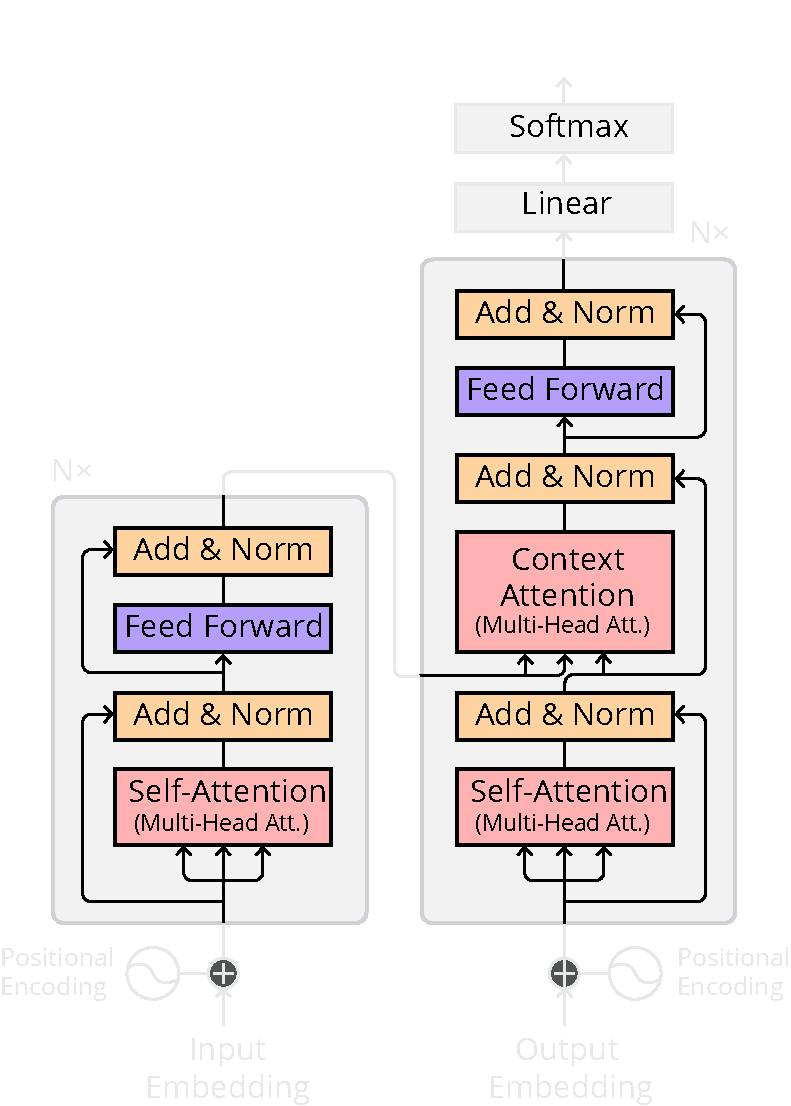
\includegraphics[width=0.9\columnwidth]{figures/transformer_mybg}
%     \tikz[baseline,remember picture]{\node[anchor=base] (t1){};}
%     \end{center}
%     \end{column}
%     \end{columns}

%     \begin{tikzpicture}[remember picture,overlay]   %% use here too
%         \uncover<2>{\path[draw=magenta,ultra thick,->](
%             [xshift=2mm,yshift=1mm]n1.north) to [out=6cm,in=0,distance=-1.5cm] ([xshift=-5.13cm,yshift=2.0cm]t1.north);}
%         \uncover<3>{\path[draw=magenta,ultra thick,->](
%             [xshift=2mm,yshift=1mm]n2.north) to [out=6cm,in=0,distance=-3cm] ([xshift=-2.67cm,yshift=2.0cm]t1.north);}
%         \uncover<4>{\path[draw=magenta,ultra thick,->](
%             [xshift=2mm,yshift=1mm]n3.north) to [out=-6cm,in=0,distance=-2.5cm] ([xshift=-2.67cm,yshift=3.55cm]t1.north);}
%     \end{tikzpicture}
% }

% \begin{itemize}
% \item[]\uncover<6->{
%     {\color{colorEntmax} Key idea:} replace softmax in attention heads by a sparse normalizing function! \quad\emoji{palms}
% }

% \bigskip

% \item[]\uncover<7->{
%     {\color{myDarkYellow} Another key idea:}
%     use a normalizing function that is adaptively sparse via a learnable $\alpha$! \quad\emoji{palms}\enspace\emoji{palms}\enspace\emoji{palms}
% }
% \end{itemize}

% % \bigskip

% % \begin{itemize}
% % \uncover<4->{\item Recall: $\alpha$ controls propensity to sparsity}
% % \uncover<5->{\item Learn each $\alpha \in [1,2]$ {\bf adaptively}!}
% % \uncover<6->{\item One $\alpha$ for each attention head and each layer}
% % \uncover<7->{\item Heads can be dense or sparse, depending on their roles.}
% % \end{itemize}

% \end{frame}

% \begin{frame}[fragile]
%     \frametitle{Related Work: Other Sparse Transformers}
%     \cornercite{Child2019,Sukhbaatar2019}

%     \vspace{-1.5cm}
%     \begin{center}
%     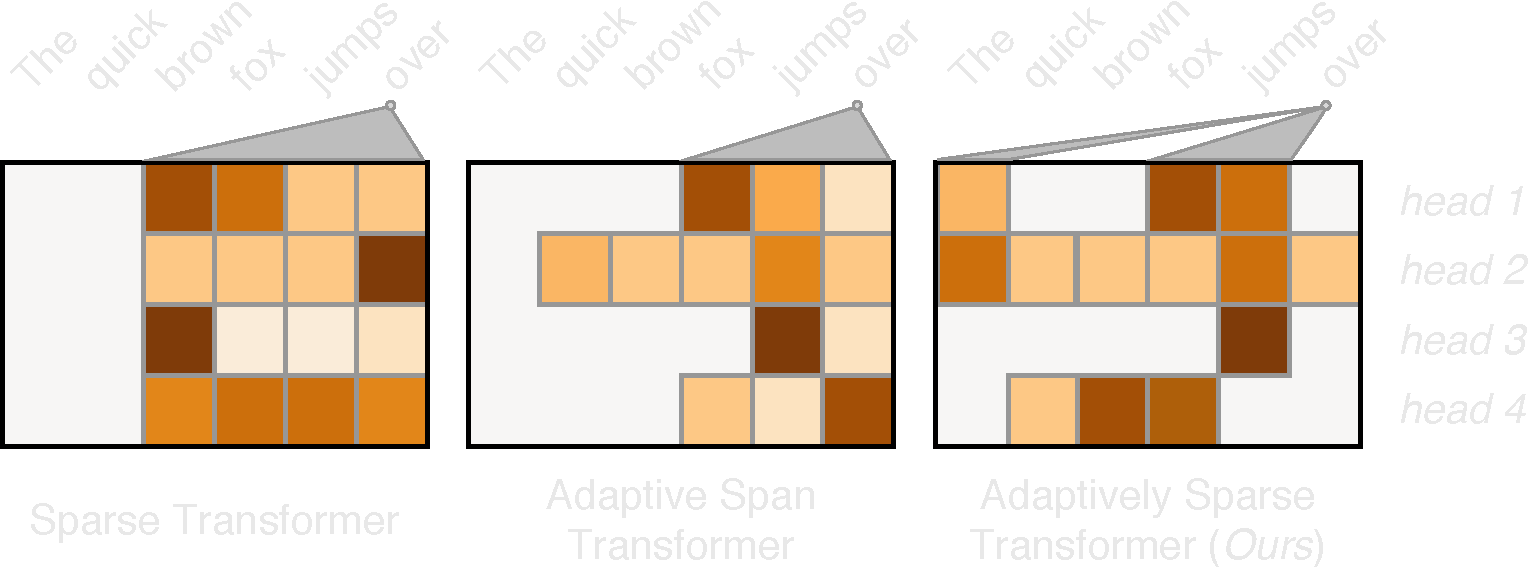
\includegraphics[width=0.7\columnwidth]{figures/comparison_mybg}

%     \bigskip

%     Our model allows {\color{myDarkYellow} non-contiguous} attention for each head.
%     \end{center}

% \end{frame}

% \section{Sparse Transformations}

% \begin{frame}[plain,t,fragile]%
%     \frametitle{What is softmax?}%
%     \centering \fontsize{12pt}{15}\selectfont
%     Softmax exponentiates and normalizes:\quad
%     $\displaystyle
%     \softmax(\xx_i) \defeq \frac{\exp \left(\xx_i\right)}{\sum_j \exp \left(\xx_j\right)}$

%     \uncover<2->{
%     {\color{myDarkYellow} It's fully dense: $\softmax(\vectsymb{z}) > \vect{0}$}}

%     \vspace{1cm}

%     \uncover<3->{Argmax can be written as:\\
%     \vspace{0.5cm}
%     $\displaystyle
%     \argmaxbf(\vectsymb{z}) \defeq \arg\max_{\vectsymb{p} \in \triangle} \DP{\vectsymb{z}}{\vectsymb{p}}$

%     \bigskip

%     \begin{itemize}
%     \item<4-> Retrieves a {\bf one-hot vector} for the highest scored index.
%     \item<5-> Sometimes used as hard attention, but not differentiable!
%     \end{itemize}
%     }
% \end{frame}

% \begin{frame}{$\Omega$-Regularized Argmax}
%     \cornercite{Niculae2017}
%     \fontsize{12pt}{15}\selectfont
%     \vspace{-0.5cm}
%     \begin{itemize}
%     \item[] For convex $\Omega$, define the {\bf $\Omega$-regularized argmax transformation}:\\
%     \bigskip
%     \begin{center}
%     $\displaystyle
%     \argmaxbf{}_{{\Omega}}(\vectsymb{z}) \defeq \arg\max_{\vectsymb{p} \in \triangle} \DP{\vectsymb{z}}{\vectsymb{p}} {\color{tPeony}- \Omega(\vectsymb{p})}$
%     \end{center}
%     \end{itemize}
%     \bigskip
%     \begin{itemize}
%     \uncover<2->{\item {\color{myDarkYellow} Argmax} corresponds to {\bf no regularization}, $\displaystyle\Omega \equiv 0$}
%     \uncover<3->{\item {\color{myDarkYellow} Softmax} amounts to {\bf entropic regularization}, $\displaystyle\Omega(\vectsymb{p}) = \sum_{i=1}^K p_i \log p_i$}
%     \uncover<4->{\item {\color{myDarkYellow} Sparsemax} amounts to {\bf $\ell_2$-regularization}, $\displaystyle\Omega(\vectsymb{p}) = \frac{1}{2}\|\vectsymb{p}\|^2$.}
%     \end{itemize}
%     \bigskip
%     \begin{itemize}
%     \item[] \uncover<5->{Is there something in-between?}
%     \end{itemize}
%     \uncover<4>{\cornercite[south east]{sparsemax}}
% \end{frame}

% \begin{frame}{$\alpha$-Entmax}
%     \cornercite{Peters2019ACL}
%     \vspace{-1cm}
%     \fontsize{12pt}{15}\selectfont
%     \begin{itemize}
%     \item[] Parametrized by {\color{tPeony}$\alpha \ge 0$}:
%     \end{itemize}
%     \bigskip
%     \begin{center}
%     $\displaystyle
%     \Omega_{{\color{tPeony}\alpha}}(\vectsymb{p}) \defeq 
%     \left\{
%     \begin{array}{ll}
%     \frac{1}{\alpha(\alpha-1)} \left(1 - \sum_{i=1}^K p_i^{\alpha}\right) & \text{if $\alpha \ne 1$}\\
%     \sum_{i=1}^K p_i\log p_i & \text{if $\alpha = 1$.}
%     \end{array}
%     \right.$
%     \end{center}
%     \bigskip
%     \begin{itemize}
%         \uncover<2->{\item {\bf Argmax} corresponds to {\color{tPeony}$\alpha \rightarrow \infty$}}
%         \uncover<3->{\item {\bf Softmax} amounts to {\color{tPeony}$\alpha \rightarrow 1$}}
%         \uncover<4->{\item {\bf Sparsemax} amounts to {\color{tPeony}$\alpha = 2$}.}
%     \end{itemize}
%     \bigskip
%     \begin{itemize}
%         \uncover<5->{\item[] {\color{myDarkYellow} Key result:} {\bf can be sparse for $\alpha > 1$}, propensity for sparsity increases with $\alpha$.}
%     \end{itemize}

% \end{frame}

% \section{Efficient Marginalization of Discrete and Structured Latent Variables via Sparsity}

% \begin{frame}
%     \frametitle{Learning $\alpha$}

%     \begin{itemize}
%         \uncover<2->{\item[] {\color{myDarkYellow} Key contribution}: \\\bigskip\quad a closed-form expression for $\pfrac{\aentmax(\x)}{\alpha}$ \quad\emoji{oface}}
%     \end{itemize} 

%     \bigskip

%     \begin{itemize}

%         \uncover<3->{\item[] Requires argmin differentiation $\rightarrow$ see paper for details!}

%     \end{itemize}

%     \uncover<4->{\overlaybox[0.5]{\texttt{:pip install entmax}\\Check \href{https://github.com/deep-spin/entmax}{\tt github.com/deep-spin/entmax}}}

% \end{frame}

% \begin{frame}
%     \frametitle{BLEU Scores}

%     \begin{table}[ht]
%         \begin{center}
%         \small
%         \resizebox{0.8\columnwidth}{!}{\begin{tabular}{lrrrr}
%         \toprule
%         activation
%         & \langp{de}{en} & \langp{ja}{en}
%         & \langp{ro}{en} & \only<1>{\langp{en}{de}}\only<2->{{\color{tPeony} \langp{en}{de}}}\\
%         \midrule
%         $\softmaxlight$
%         & 29.79
%         & 21.57
%         & 32.70
%         & 26.02 \\
%         $\aentmax[1.5]$
%         & 29.83
%         & {\color{myDarkYellow} 22.13}
%         & {\color{myDarkYellow} 33.10}
%         & 25.89 \\
%         $\aentmax[\alpha]$
%         & {\color{myDarkYellow} 29.90}
%         & 21.74
%         & 32.89
%         & {\color{myDarkYellow} 26.93} \\
%         \bottomrule
%         \end{tabular}}
%         \end{center}
%     \end{table}

%     \bigskip

%     \begin{itemize}
%         \uncover<3>{\item[] For analysis for other language pairs, see Appendix A.}
%     \end{itemize}

% \end{frame}

% \section{Conclusions}

% \begin{frame}[fragile]
%   \frametitle{Key Takeaways}

%     \centering\fontsize{14pt}{14}\selectfont%
%     Introduce {\color{myDarkYellow} adaptive} sparsity\\
%     for Transformers via $\alpha$-entmax with a {\color{myDarkYellow}gradient learnable $\alpha$}.
%     %
%     %
%     \vfill
%     %
%     %
%     \begin{columns}[T]
%     \small
%     \begin{column}{.33\textwidth}
%     \centering
%     \uncover<2->{
%     \textbf{\emph{adaptive sparsity}}\\[.5\baselineskip]
%     \vspace{0.2cm}
%     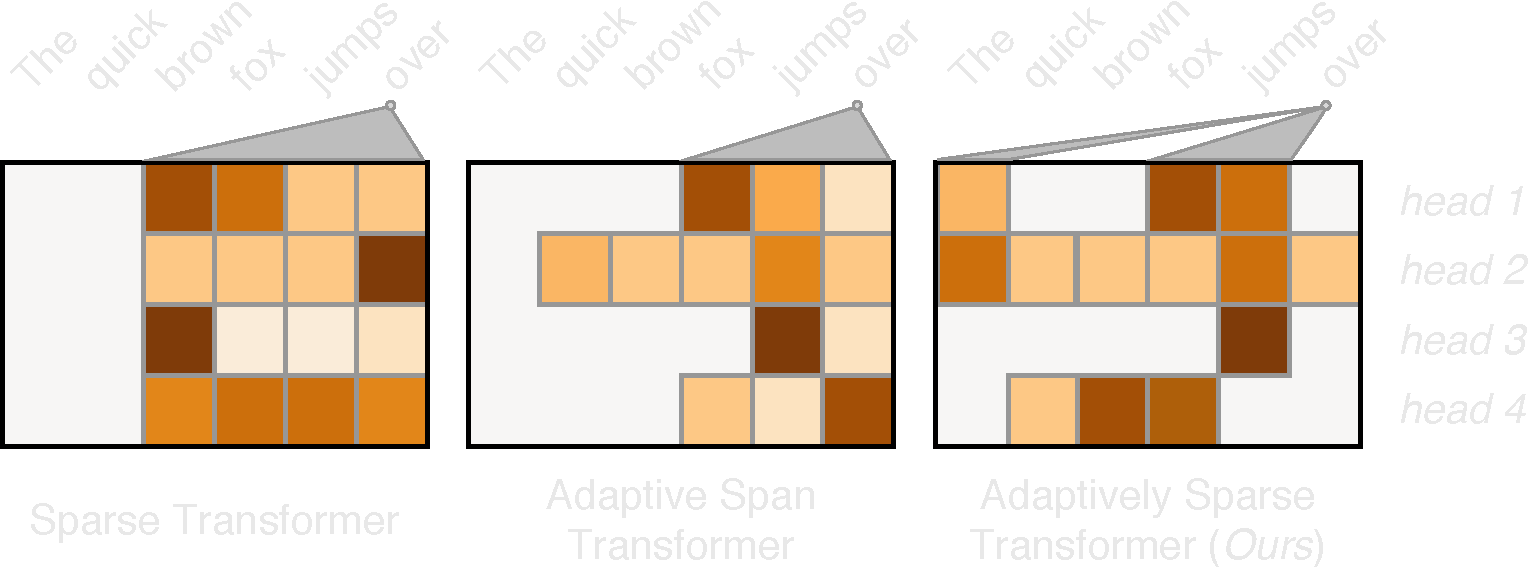
\includegraphics[trim=157mm 17mm 0 0, clip, width=.7\textwidth]{figures/comparison_mybg}}%
%     \end{column}
%     \begin{column}{.33\textwidth}
%     \centering
%     \uncover<3->{
%     \textbf{\emph{reduced head redundancy}}\\[\baselineskip]}
%     \vspace{-0.2cm}
%     \begin{tikzpicture}[node distance=1.5ex,font=\scriptsize,scale=0.5, visible on=<3->]

%         \definecolor{color0}{rgb}{0.12156862745098,0.466666666666667,0.705882352941177}
%         \definecolor{color1}{rgb}{1,0.498039215686275,0.0549019607843137}
%         \definecolor{color2}{rgb}{0.172549019607843,0.627450980392157,0.172549019607843}
        
%         \begin{groupplot}[group style={group size=1 by 1}]
%         \nextgroupplot[
%         legend cell align={left},
%         legend style={
%                 nodes={scale=1.1, transform shape}, at={(0.97,0.2)}, anchor=east, draw=white!80.0!black, fill=myfg!30!mybg},
%         tick align=outside,
%         tick pos=left,
%         x grid style={white!69.01960784313725!black},
%         xmin=0.5, xmax=6.5,
%         xtick = {1, 2, 3, 4, 5, 6},
%         xtick style={color=white},
%         y grid style={white!69.01960784313725!black},
%         ymin=0.1, ymax=0.7,
%         ytick = {0.2, 0.4, 0.6},
%         ytick style={color=white}
%         ]
%         \addplot [thick, color0, mark=square*, mark size=3, mark options={solid}]
%         table {%
%         1 0.38571667343747
%         2 0.402429158203537
%         3 0.440747738282957
%         4 0.359233941813858
%         5 0.337470844946825
%         6 0.339900884621234
%         };
%         \addlegendentry{softmax}
%         \addplot [thick, color1, mark=*, mark size=3, mark options={solid}]
%         table {%
%         1 0.378367748537659
%         2 0.504354104995477
%         3 0.573529792473815
%         4 0.525266398541884
%         5 0.439669581263257
%         6 0.421346772557364
%         };
%         \addlegendentry{1.5-entmax}
%         \addplot [thick, color2, mark=asterisk, mark size=3, mark options={solid}]
%         table {%
%         1 0.427742934860258
%         2 0.484287995253192
%         3 0.533714455762104
%         4 0.449772918584636
%         5 0.3935698561848
%         6 0.355665944457941
%         };
%         \addlegendentry{$\alpha$-entmax}
%     \end{groupplot}
%     \end{tikzpicture}
%     \end{column}
%     \begin{column}{.33\textwidth}
%     \centering
%     \uncover<4->{
%     \textbf{\emph{clearer head roles}}\\[\baselineskip]
%     \vspace{-0.2cm}
%     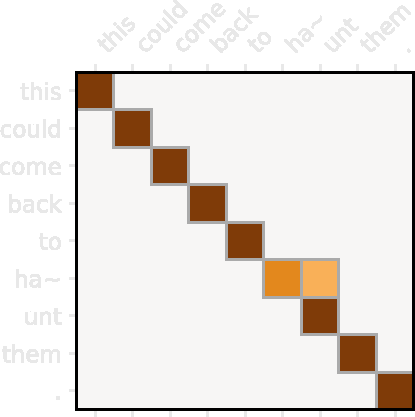
\includegraphics[width=.6\textwidth]{figures/bpe4}}
%     \end{column}
%     \end{columns}

%     \vfill

%     \centering
%     {\scriptsize
%     \color{mygr}
%     \begin{tabular}{r@{~}l@{\quad}r@{~}l}
%     \raisebox{-0.7mm}[\height][\depth]{\emoji{githubfg}}& \href{https://github.com/deep-spin/entmax}{\tt github.com/deep-spin/entmax} &
%     \raisebox{-0.4mm}[\height][\depth]{\emoji{home}}& \href{https://goncalomcorreia.github.io}{\tt goncalomcorreia.github.io}
%     \end{tabular}}

% \end{frame}

% \begin{frame}
%     \centering
%     \vspace{-2cm}
%     \fontsize{30pt}{15}\selectfont
%     Thank you!

%     \bigskip

%     \fontsize{20pt}{15}\selectfont
%     Questions?

%     \overlaybox[0.7]{\texttt{:pip install entmax}\\Check \href{https://github.com/deep-spin/entmax}{\tt github.com/deep-spin/entmax}}
% \end{frame}

% {
% \setbeamercolor{background canvas}{bg=white}
% \setbeamercolor{normal text}{fg=mygr}
% \setbeamercolor{frametitle}{fg=mybg}
% \usebeamercolor[fg]{frametitle}
% \usebeamercolor[fg]{normal text}
% \begin{frame}
% \frametitle{Acknowledgements}
% \centering
% \small
% 
\includegraphics[width=.2\textwidth]{img/erc.png}\\
% This work was supported by the European Research
% Council (ERC StG DeepSPIN 758969) and by the
% Fundação para a Ciência e Tecnologia through contract UID/EEA/50008/2019 and
% CMUPERI/TIC/0046/2014 (GoLocal).
% \end{frame}
% }

\begin{frame}[t,allowframebreaks]
\frametitle{References}
\printbibliography
\end{frame}

\end{document}

